\documentclass[aspectratio=169]{beamer}
\usepackage{lectureppt} % Load your custom style


\title{수리경제학}
\subtitle{미분 - 중간고사 대비 Review}
\author{이재석}
\date{2025-04-17 \\ (updated:\today)}

\begin{document}

\begin{frame}
  \titlepage
\end{frame}

\begin{frame}{목차}
  \tableofcontents
\end{frame}

% \section{미분을} % 정의하는 방법 1 대수학 (Algebra)적 접근}
% \begin{frame}%{미분을 정의하는 방법 1: 대수학 (Algebra)적 접근}
%   \begin{itemize}
%     \item 함수 \( f(x) \)의 미분계수는 다음과 같이 정의됨
%     % \[ f'(x)=\lim_{h \to 0} \frac{f(x+h)-f(x)}{h} \]
%     \item 이 정의는 함수의 기울기를 나타내며, 접선의 기울기와 관련됨
%   \end{itemize}

% 제일 쉽고 간편하게 개념을 느끼고 사용하면 됨.
% 크게 세가지로 보여 줄 수 있음. 1. 대수학적으로 보여주기 2.기하학적적으로 보여주기 3.수학적 명제로 증명하기.
% 수학적 명제가 가장 완결성을 가지지만 추상적이기 때문에 '느끼기'힘듦.
% 대수학적으로 보여주고, 기하학적으로 보여주고, 다시 대수학적으로 살펴볼 것.
% 우리의 목적은 수하적으로 완결한 미분을 배우는것이 아니라, 아래 문제를 풀기 위함임.
% 1.효용극대화 2.이윤극대화 3.비용최소화
% 이 문제들은 미분을 통해 풀 수 있음.




\section{극한}

\begin{frame}{극한}
  \begin{definition}[도함수]
    실수($\mathbb{R}$)의 어떤 함수 \textcolor{violet}{$f(x)$}가 정의되는 포인트 \textcolor{blue}{\emph{$a$}} 에서 \emph{미분가능(differentiable)} 하고, 정의역이 포인트 \textcolor{blue}{\emph{$a$}} 를 포함한다면, \textcolor{blue}{\emph{$a$}} 에서 \textcolor{red}{미분계수(순간변화율)} \textcolor{red}{\emph{$L$}} 은 \\
    \begin{equation}
      \textcolor{red}{L} = \textcolor{teal}{\lim_{h \to 0} \frac{f(\textcolor{blue}{a}+h)-f(\textcolor{blue}{a})}{h}}
    \end{equation}
  \end{definition}
  \textcolor{red}{미분계수}는, 포인트 \textcolor{blue}{\emph{$a$}} 에서 극한값. 올바른 \textcolor{red}{$L$} 값을 구하기 위해서는, 극한의 성질을 이해해야 함. \\또한, 당연하게도 미분가능성의 조건은 포인트 \textcolor{blue}{\emph{$a$}} 에서 올바른 극한값의 조건을 만족해야 함.
\end{frame}



\begin{frame}{여러 함수형태에 따른 극한값}
  % Top Row: Two images
  \begin{columns}
    \begin{column}{0.5\textwidth}
      \centering
      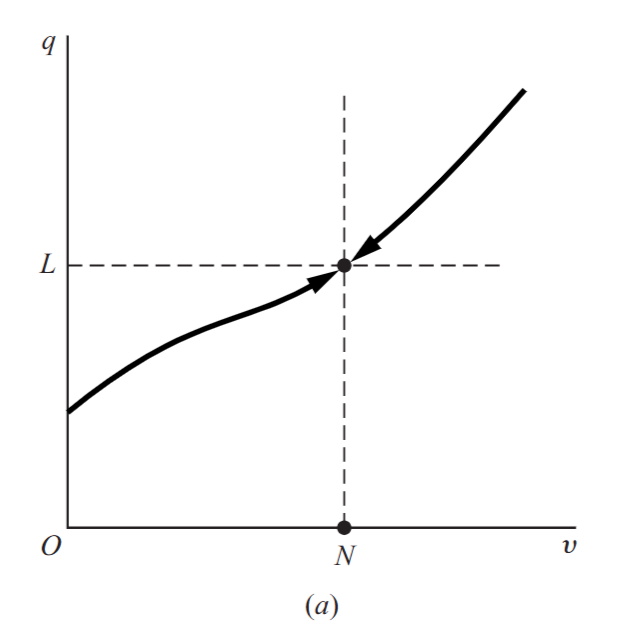
\includegraphics[width=\linewidth,height=0.48\textheight,keepaspectratio]{../fig/limits_illustration_a.png}
    \end{column}
    \begin{column}{0.5\textwidth}
      \centering
      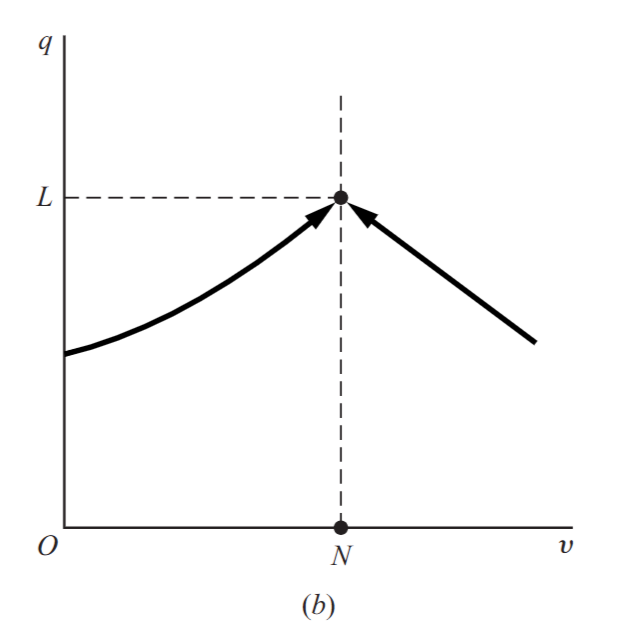
\includegraphics[width=\linewidth,height=0.48\textheight,keepaspectratio]{../fig/limits_illustration_b.png}
    \end{column}
  \end{columns}

  \vspace{1em}

  % Bottom Row: Two text blocks
  \begin{columns}
    \begin{column}{0.5\textwidth}
      \footnotesize
      \textbf{\emph{극한값이 존재}}\\
      \small \textcolor{violet}{$f(\cdot)$}는 'smooth'한 곡선.\\
      좌측에서 \textcolor{blue}{$N$}으로 접근하거나, 우측에서 접근할 시, 모두 극한값이 \textcolor{red}{\emph{L}}로 수렴.
    \end{column}
    \begin{column}{0.5\textwidth}
      \footnotesize
      \textbf{\emph{극한값이 존재}}\\
      \small \textcolor{violet}{$f(\cdot)$}는 'smooth'하지 \textcolor{magenta}{않는} 곡선.\\
      하지만, 좌측에서 \textcolor{blue}{$N$}으로 접근하거나, 우측에서 접근할 시, 모두 극한값이 \textcolor{red}{\emph{L}}로 수렴.
    \end{column}
  \end{columns}
\end{frame}



\begin{frame}{여러 함수형태에 따른 극한값}

  % Top row: two images
  \begin{columns}
    \begin{column}{0.5\textwidth}
      \centering
      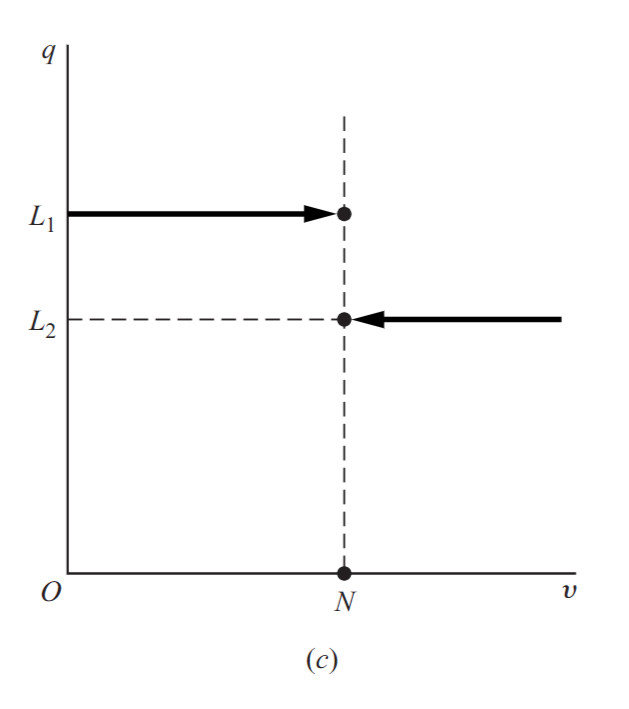
\includegraphics[width=\linewidth,height=0.48\textheight,keepaspectratio]{../fig/limits_illustration_c.png}
    \end{column}
    \begin{column}{0.5\textwidth}
      \centering
      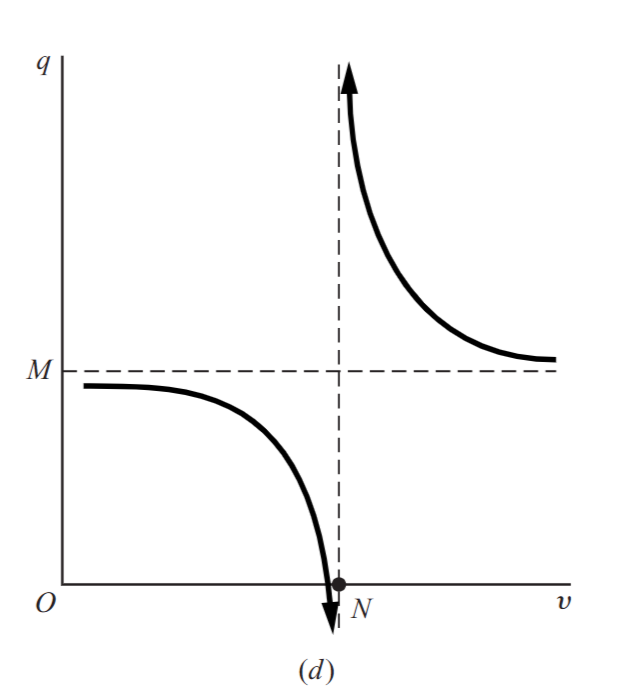
\includegraphics[width=\linewidth,height=0.48\textheight,keepaspectratio]{../fig/limits_illustration_d.png}
    \end{column}
  \end{columns}

  \vspace{0.5em}

  % Bottom row: two descriptions
  \begin{columns}
    \begin{column}{0.5\textwidth}
      \footnotesize
      \textbf{\emph{극한값이 존재하지 \textcolor{magenta}{않음}}}\\
      \scriptsize \textcolor{violet}{$f(\cdot)$}는 'smooth'하지 \textcolor{magenta}{않는} 곡선.\\
      좌측에서 \textcolor{blue}{$N$}으로 접근시 극한값 $L_1$, 우측에서 접근할 시 극한값 $L_2$.\\
      극한값 \textcolor{red}{\emph{L}}이 존재하지 않음.
    \end{column}
    \begin{column}{0.5\textwidth}
      \footnotesize
      \textbf{\emph{극한값이 존재하지 \textcolor{magenta}{않음}}}\\
      \scriptsize \textcolor{violet}{$f(\cdot)$}는 'smooth'한 곡선.\\
      좌측에서 극한값 $-\infty$, 우측에서 극한값 $\infty$.\\
      따라서 \textcolor{red}{\emph{L}}이 존재하지 않음.
    \end{column}
  \end{columns}

\end{frame}





\begin{frame}{함수의 극한: $f(x) = ax$ 의 형태}
  \scriptsize
  \begin{columns}
    % Left column: TikZ plot
    \begin{column}{0.55\textwidth}
      \centering
      
      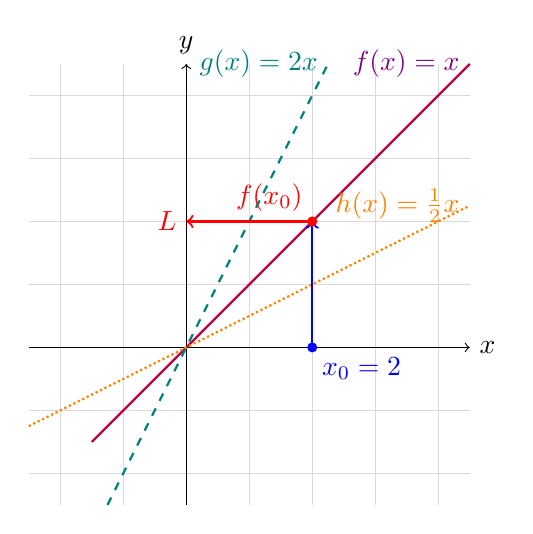
\begin{tikzpicture}[scale=0.8]
        % Grid
        \draw[step=1cm,gray,very thin,opacity=0.3] (-2.5,-2.5) grid (4.5,4.5);
      
        % Axes
        \draw[->] (-2.5,0) -- (4.5,0) node[right] {$x$};
        \draw[->] (0,-2.5) -- (0,4.5) node[above] {$y$};

        % f(x) = x
        \draw[thick,purple] (-1.5,-1.5) -- (4.5,4.5) node[left] {\textcolor{violet}{$f(x) = x$}};
        
        % g(x) = 2x
        \draw[thick,teal,dashed] (-1.25,-2.5) -- (2.25,4.5) node[left] { \textcolor{teal}{$g(x) = 2x$}};

        % h(x) = (1/2)x
        \draw[thick,orange,densely dotted] (-2.5, -1.25) -- (4.5,2.25) node[left] {\textcolor{orange}{$h(x) = \frac{1}{2}x$}};
      
        % Blue dot at a = 2
        \filldraw[blue] (2,0) circle (2pt) node[below right] {$x_0=2$};
        \draw[->,blue,thick] (2,0) -- (2,2);
        
        % Red dot at f(a)
        \filldraw[red] (2,2) circle (2pt) node[above left] {$f(x_0)$};
        \draw[->,red,thick] (2,2) -- (0,2);
        \node[red, left] at (0,2) {$L$};
      \end{tikzpicture}
    \end{column}

    % Right column: description
    \begin{column}{0.45\textwidth}
      \begin{itemize}
        \item $\lim_{x \to 2} \textcolor{violet}{f(x)} = 2$ \\
          $\lim_{x \to 2} \textcolor{teal}{g(x)} = 4$ \\
          $\lim_{x \to 2} \textcolor{orange}{h(x)} = 1/2$
        \item $\lim_{x \to 0} \textcolor{violet}{f(x)} = 0 $ \\
          $\lim_{x \to 0} \textcolor{teal}{g(x)} = 0 $ \\
          $\lim_{x \to 0} \textcolor{orange}{h(x)} = 0 $
        \item $\lim_{x \to \infty} \textcolor{violet}{f(x)} = \infty $ \\
          $\lim_{x \to \infty} \textcolor{teal}{g(x)} = \infty $ \\
          $\lim_{x \to \infty} \textcolor{orange}{h(x)} = \infty $
        \item $\lim_{x \to -\infty} \textcolor{violet}{f(x)} = -\infty $ \\
          $\lim_{x \to -\infty} \textcolor{teal}{g(x)} = -\infty $ \\
          $\lim_{x \to -\infty} \textcolor{orange}{h(x)} = -\infty $
      \end{itemize}
    \end{column}
  \end{columns}
\end{frame}

\begin{frame}{함수의 극한: $f(x) = \dfrac{a}{x}$ 의 형태}
  \scriptsize
  \begin{columns}
    % Left column: TikZ plot
    \begin{column}{0.55\textwidth}
      \centering
      \begin{tikzpicture}[scale=0.65, domain=-4.2:-0.2, samples=100]
        % Grid
        \draw[step=1cm,gray,very thin,opacity=0.3] (-4.5,-4.5) grid (4.5,4.5);

        % Axes
        \draw[->] (-4.5,0) -- (4.5,0) node[right] {$x$};
        \draw[->] (0,-4.5) -- (0,4.5) node[above] {$y$};

        % f(x) = 1/2x → violet
        \draw[thick,violet,densely dotted, domain=-4.2:-0.2] plot (\x, {0.5/\x});
        \draw[thick,violet,densely dotted, domain=0.2:4.2] plot (\x, {0.5/\x}) 
          node[below left] {\textcolor{violet}{$f(x)=\dfrac{1}{2x}$}};

        % g(x) = 1/x → teal
        \draw[thick,teal,dash pattern=on 4pt off 2pt, domain=-4.2:-0.3] plot (\x, {1/\x});
        \draw[thick,teal,dash pattern=on 4pt off 2pt, domain=0.3:4.2] plot (\x, {1/\x}) 
          node[right] {\textcolor{teal}{$g(x)=\dfrac{1}{x}$}};

        % h(x) = 2/x → orange
        \draw[thick,orange,dashed, domain=-4.2:-0.5] plot (\x, {2/\x});
        \draw[thick,orange,dashed, domain=0.5:4.2] plot (\x, {2/\x}) 
          node[above right] {\textcolor{orange}{$h(x)=\dfrac{2}{x}$}};

        % s(x) = 3/x remains purple (unchanged)
        \draw[thick,purple, domain=-4.2:-0.7] plot (\x, {3/\x});
        \draw[thick,purple, domain=0.7:4.2] plot (\x, {3/\x}) 
          node[above left] {\textcolor{purple}{$s(x)=\dfrac{3}{x}$}};

        % Vertical dashed line at x = 0 (asymptote)
        \draw[gray, dashed] (0,-4.5) -- (0,4.5);
      \end{tikzpicture}
    \end{column}

    % Right column: description
    \begin{column}{0.45\textwidth}
      \begin{itemize}
        \item $\lim_{x \to 1} \textcolor{violet}{f(x)} = \frac{1}{2}$ \\
              $\lim_{x \to 1} \textcolor{teal}{g(x)} = 1$ \\
              $\lim_{x \to 1} \textcolor{orange}{h(x)} = 2$
        \item $\lim_{x \to 0^+} \textcolor{violet}{f(x)} = \infty $ \\
              $\lim_{x \to 0^+} \textcolor{teal}{g(x)} = \infty $ \\
              $\lim_{x \to 0^+} \textcolor{orange}{h(x)} = \infty $
        \item $\lim_{x \to 0^-} \textcolor{violet}{f(x)} = -\infty $ \\
              $\lim_{x \to 0^-} \textcolor{teal}{g(x)} = -\infty $ \\
              $\lim_{x \to 0^-} \textcolor{orange}{h(x)} = -\infty $
        \item $\lim_{x \to \infty} \textcolor{violet}{f(x)} = 0 $ \\
              $\lim_{x \to \infty} \textcolor{teal}{g(x)} = 0 $ \\
              $\lim_{x \to \infty} \textcolor{orange}{h(x)} = 0 $
        \item $\lim_{x \to -\infty} \textcolor{violet}{f(x)} = 0^- $ \\
              $\lim_{x \to -\infty} \textcolor{teal}{g(x)} = 0^- $ \\
              $\lim_{x \to -\infty} \textcolor{orange}{h(x)} = 0^- $
        % \item 모든 함수는 $\displaystyle f(x)=\frac{a}{x}$ 꼴이며 $x \ne 0$에서 정의됨.
        % \item $x \to \infty$일 때 $\displaystyle f(x) \to 0$
        % \item $x \to 0^+$ 또는 $x \to 0^-$일 때 수직선 방향에 따라 극한은 $\pm \infty$
        % \item $\displaystyle \lim_{x \to \infty} \frac{a}{x} = 0$ \\
        %       $\displaystyle \lim_{x \to 0^+} \frac{a}{x} = \infty$ (if \( a > 0 \)) \\
        %       $\displaystyle \lim_{x \to 0^-} \frac{a}{x} = -\infty$
        % \item 계수 \( a \)가 커질수록 그래프가 더 가파르게 생김
      \end{itemize}
      % \vspace{0.3em}
      % \textcolor{gray}{\scriptsize 수직 점근선: $x=0$, 수평 점근선: $y=0$}
    \end{column}
  \end{columns}
\end{frame}





\begin{frame}{함수의 극한: $f(x) = x^a$ 의 형태}
  \scriptsize
  \begin{columns}
    % Left column: TikZ plot
    \begin{column}{0.55\textwidth}
      \centering
      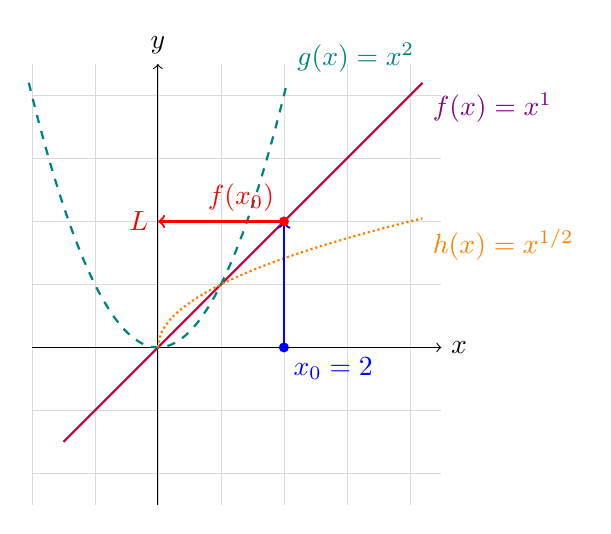
\begin{tikzpicture}[scale=0.8, domain=-1.5:4.2, samples=100]
        % Grid
        \draw[step=1cm,gray,very thin,opacity=0.3] (-2,-2.5) grid (4.5,4.5);
        
        % Axes
        \draw[->] (-2,0) -- (4.5,0) node[right] {$x$};
        \draw[->] (0,-2.5) -- (0,4.5) node[above] {$y$};

        % f(x) = x^1
        \draw[thick,purple] plot (\x, {\x}) node[below right] {\textcolor{violet}{$f(x)=x^1$}};

        % g(x) = x^2 with codomain suppressed to y <= 4.2
        \draw[thick,teal,dashed, domain=-2.05:2.05] plot (\x, {\x*\x}) node[above right] {\textcolor{teal}{$g(x)=x^2$}};

        % h(x) = sqrt(x)
        \draw[thick,orange,densely dotted, domain=0:4.2] plot (\x, {sqrt(\x)}) node[below right] {\textcolor{orange}{$h(x)=x^{1/2}$}};
        
        % Blue vertical line at x = 2
        \filldraw[blue] (2,0) circle (2pt) node[below right] {$x_0=2$};
        \draw[->,blue,thick] (2,0) -- (2,2);

        % Red dot at f(2) = 2
        \filldraw[red] (2,2) circle (2pt) node[above left] {$f(x_0)$};
        \draw[->,red,thick] (2,2) -- (0,2);
        \node[red, left] at (0,2) {$L$};
      \end{tikzpicture}
    \end{column}

    % Right column: description
    \begin{column}{0.45\textwidth}
      \begin{itemize}
        \item $\lim_{x \to 2} \textcolor{violet}{f(x)} = 2$ \\
          $\lim_{x \to 2} \textcolor{teal}{g(x)} = 4$ \\
          $\lim_{x \to 2} \textcolor{orange}{h(x)} = \sqrt{2}$
        \item $\lim_{x \to 0} \textcolor{violet}{f(x)} = DNE$\\
          $\lim_{x \to 0} \textcolor{teal}{g(x)} = 0$\\
          $\lim_{x \to 0} \textcolor{orange}{h(x)} = 0$
        \item $\lim_{x \to \infty} \textcolor{violet}{f(x)} = \infty $ \\
          $\lim_{x \to \infty} \textcolor{teal}{g(x)} = \infty $ \\
          $\lim_{x \to \infty} \textcolor{orange}{h(x)} = \infty $
        \item $\lim_{x \to -\infty} \textcolor{violet}{f(x)} = -\infty $ \\
          $\lim_{x \to -\infty} \textcolor{teal}{g(x)} = \infty $ \\
          $\lim_{x \to -\infty} \textcolor{orange}{h(x)} = DNE $
        \item $\lim_{x \to 0^+} \textcolor{violet}{f(x)} = 0$ \\
          $\lim_{x \to 0^+} \textcolor{teal}{g(x)} = 0$ \\
          $\lim_{x \to 0^+} \textcolor{orange}{h(x)} = 0$ 
      \end{itemize}
      % \vspace{0.3em}
      % \textcolor{gray}{\scriptsize($x > 0$ 영역에서 정의된 함수들 비교 — 특히 $x^{1/2}$는 $x < 0$에서는 정의되지 않음.)}
    \end{column}
  \end{columns}
\end{frame}




\begin{frame}{함수의 극한: $f(x) = a^x$ 의 형태}
  \scriptsize
  \begin{columns}
    % Left column: TikZ plot
    \begin{column}{0.55\textwidth}
      \centering
      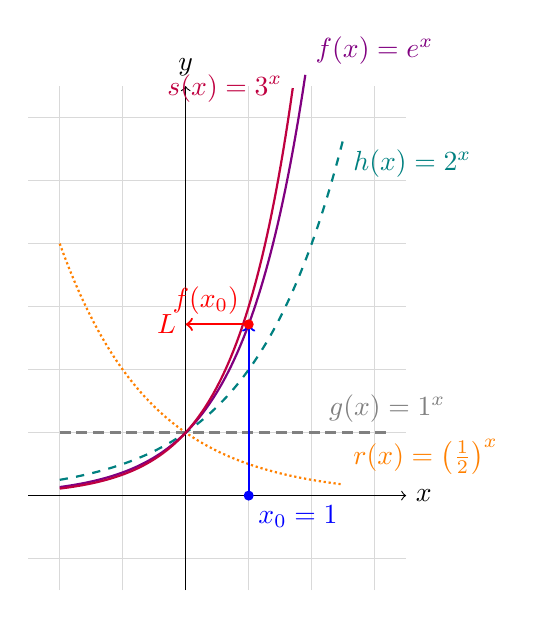
\begin{tikzpicture}[scale=0.8, domain=-2:2.5, samples=100]
        % Grid
        \draw[step=1cm,gray,very thin,opacity=0.3] (-2.5,-1.5) grid (3.5,6.5);
        
        % Axes
        \draw[->] (-2.5,0) -- (3.5,0) node[right] {$x$};
        \draw[->] (0,-1.5) -- (0,6.5) node[above] {$y$};

        % r(x) = (1/2)^x
        \draw[thick,orange,densely dotted] plot (\x, {pow(0.5,\x)}) node[above right] {\textcolor{orange}{$r(x)=\left(\frac{1}{2}\right)^x$}};

        % g(x) = 1^x (constant 1)
        \draw[thick,gray,dash pattern=on 4pt off 2pt] (-2,1) -- (3.2,1) node[above] {\textcolor{gray}{$g(x)=1^x$}};

        % h(x) = 2^x
        \draw[thick,teal,dashed] plot (\x, {pow(2,\x)}) node[below right] {\textcolor{teal}{$h(x)=2^x$}};

        % f(x) = e^x
        \draw[thick,violet, domain=-2:1.9] plot (\x, {exp(\x)}) node[above right] {\textcolor{violet}{$f(x)=e^x$}};

        % s(x) = 3^x
        \draw[thick,purple, domain=-2:1.7] plot (\x, {pow(3,\x)}) node[left] {\textcolor{purple}{$s(x)=3^x$}};

        % Reference vertical line at x = 1
        \filldraw[blue] (1,0) circle (2pt) node[below right] {$x_0=1$};
        \draw[->,blue,thick] (1,0) -- (1,{exp(1)});
        \filldraw[red] (1,{exp(1)}) circle (2pt) node[above left] {$f(x_0)$};
        \draw[->,red,thick] (1,{exp(1)}) -- (0,{exp(1)});
        \node[red,left] at (0,{exp(1)}) {$L$};
      \end{tikzpicture}
    \end{column}

    % Right column: description
    \begin{column}{0.45\textwidth}
      % \begin{itemize}
      %   \item $\textcolor{orange}{\left(\frac{1}{2}\right)^x}$: 감소 함수, $x \to \infty$일 때 0에 수렴
      %   \item $\textcolor{gray}{1^x}$: 항상 1 (상수함수)
      %   \item $\textcolor{teal}{2^x}$: 전형적인 증가 함수
      %   \item $\textcolor{blue}{e^x}$: 미분 가능하고 자연로그의 역함수
      %   \item $\textcolor{violet}{3^x}$: 가장 빠르게 증가
      % \end{itemize}
      % \vspace{0.5em}
      \begin{itemize}
        \item $\lim_{x \to 1} \textcolor{violet}{f(x)} = e $ \\
          $\lim_{x \to 1} \textcolor{teal}{h(x)} = 2 $ \\
          $\lim_{x \to 1} \textcolor{orange}{r(x)} = 1/2 $
        \item $\lim_{x \to \infty} a^x = 
          \begin{cases}
            0 & \text{if } 0 < a < 1 \\
            1 & \text{if } a = 1 \\
            \infty & \text{if } a > 1
          \end{cases}$
        \item $\lim_{x \to -\infty} a^x = 
          \begin{cases}
            \infty & \text{if } 0 < a < 1 \\
            1 & \text{if } a = 1 \\
            0 & \text{if } a > 1
          \end{cases}$
      % \item $ \lim_{x \rightarrow x_0} \textcolor{blue}{e^x} = e^{x_0}$
      \end{itemize}
    \end{column}
  \end{columns}
\end{frame}






\section{극한의 성질}
\begin{frame}{극한의 성질}
  함수 \( y = f(x) \) 에 대해 (단, \( a \) 와 \( b \) 는 상수),
  \begin{itemize}
    \item \textbf{정리 I}  \\
    \( y = ax + b \) 일 때,  
    \( \lim_{x \to c} y = ac + b \)  
    
    \item \textbf{정리 II}  \\
    \( y = f(x) = b \) (상수 함수) 일 때,  
    \( \lim_{x \to c} y = b \)  
    % 즉, 상수 함수의 극한은 해당 상수입니다.  
    % 이는 \( a = 0 \) 인 정리 I의 특수한 경우입니다.

    \item \textbf{정리 III}  \\
    \( y = x \) 일 때, \( \lim_{x \to c} y = c \),   \\
    \( y = x^k \) 일 때, \( \lim_{x \to c} y = c^k \)  
  \end{itemize}
  % 이 세 정리에서는 \( x = c \) 를 직접 대입해 극한값을 구할 수 있지만,  이는 특수한 경우일 뿐이며, 
  \emph{*일반적으로는 “\( x \to c \)” 는 “\( x = c \)” 와 같지 않음 (대입시 다른 값).}

  % \vspace{0.5cm}

  \begin{itemize}
    \item \textbf{예시 1:} \( y = 5x + 7 \)  
    \[
      \lim_{x \to 2} y = 5(2) + 7 = 17,\quad
      \lim_{x \to 0} y = 5(0) + 7 = 7
    \]

    \item \textbf{예시 2:} \( y = x^3 \)  
    \[
      \lim_{x \to 2} y = (2)^3 = 8
    \]
  \end{itemize}
\end{frame}




\section{극한의 성질과 계산}

\begin{frame}{극한의 성질 (두 함수의 조합)}
  두 개의 함수 \( y_1 = f(x) \), \( y_2 = g(x) \) 가 \( x \) 에 대해 주어지고, 다음과 같은 유한한 실수의 극한값을 가질 때:
  \[
    \lim_{x \to c} y_1 = L_1, \quad \lim_{x \to c} y_2 = L_2
  \]
  % 여기서 \( L_1 \)과 \( L_2 \)는 유한한 실수라고 할 때, 다음 정리들이 적용됩니다.
  
  % \vspace{0.4cm}

  \begin{itemize}
    \item \textbf{정리 IV (합/차의 극한)}
    \[
      \lim_{x \to c} (y_1 \pm y_2) = L_1 \pm L_2
    \]
    % 두 함수의 합(또는 차)의 극한은, 각 함수의 극한의 합(또는 차)과 같습니다.

    % \vspace{0.2cm}
    % 예: 
    % \[
    %   \lim_{x \to c} 2y_1 = \lim_{x \to c} (y_1 + y_1) = L_1 + L_1 = 2L_1
    % \]
    % 이는 앞서 배운 \textbf{정리 I}과 일치합니다.
    
    % \vspace{0.5cm}

    \item \textbf{정리 V (곱의 극한)}
    \[
      \lim_{x \to c} (y_1 \cdot y_2) = L_1 \cdot L_2
    \]
    % 두 함수의 곱의 극한은, 각 극한값의 곱과 같습니다.

    % \vspace{0.2cm}
    % 특히, 함수의 제곱에 적용하면:
    % \[
    %   \lim_{x \to c} (y_1)^2 = L_1^2
    % \]
    % 이는 \textbf{정리 III}와 일치합니다.

    % \vspace{0.5cm}

    \item \textbf{정리 VI (나눗셈의 극한)}  
    단, \( L_2 \ne 0 \) 이어야 함
    \[
      \lim_{x \to c} \frac{y_1}{y_2} = \frac{L_1}{L_2}
    \]
    % 두 함수의 비의 극한은, 각 극한값의 비와 같습니다.  
    % 단, 분모의 극한 \( L_2 \) 가 0이 아니어야 의미가 정의됩니다.
  \end{itemize}
\end{frame}

\begin{frame}{다항식 함수의 극한}
  주어진 극한의 성질을 활용하면, 모든 다항식 함수의 극한을 쉽게 구할 수 있음.

  \vspace{0.3cm}
  일반적인 다항식 함수:
  \[
    y = f(x) = a_0 + a_1x + a_2x^2 + \cdots + a_nx^n
  \]

  \( x \to c \) 일 때, 각 항의 극한은 다음과 같음:
  \[
    \lim_{x \to c} a_0 = a_0, \quad
    \lim_{x \to c} a_1x = a_1c, \quad
    \lim_{x \to c} a_2x^2 = a_2c^2, \quad \cdots
  \]

  \vspace{0.3cm}
  따라서 전체 다항식의 극한은 다음과 같이 계산됨:
  \[
    \lim_{x \to c} f(x) = a_0 + a_1c + a_2c^2 + \cdots + a_nc^n
  \]

  % \vspace{0.3cm}
  % 즉, 극한값은 \( x = c \) 를 대입한 함수값 \( f(c) \) 와 같습니다.  
  % 이 사실은 다항식 함수의 **연속성** 개념을 이해하는 데 중요합니다.
\end{frame}


\begin{frame}{예제 1: 다항식 함수의 극한}
  함수 \( y = f(x) = x^2 - 9x + 7 \) 의 극한을 구하시오:
  \begin{itemize}
    \item[(a)] \( \lim_{x \to 0} f(x)  \)
    \vspace{0.3cm}
    \item[(b)] \( \lim_{x \to 3} f(x)  \)
    \vspace{0.3cm}
    \item[(c)] \( \lim_{x \to -1} f(x)  \)
  \end{itemize}
\end{frame}

\begin{frame}{예제 2: 곱 형태의 극한}
함수 \( y = f(x) = (x + 2)(x - 3) \) 의 극한을 구하시오:
\begin{itemize}
  \item[(a)] \( \lim_{x \to -1} f(x)  \)
  \vspace{0.3cm}
  \item[(b)] \( \lim_{x \to 0} f(x)  \)
  \vspace{0.3cm}
  \item[(c)] \( \lim_{x \to 5} f(x)  \)
\end{itemize}
\end{frame}

\begin{frame}{예제 3: 분수 함수의 극한}
함수 \( y = f(x) = \frac{3x + 5}{x + 2} \) 의 극한을 구하시오:
\begin{itemize}
  \item[(a)] \( \lim_{x \to 0} f(x)  \)
  \vspace{0.3cm}
  \item[(b)] \( \lim_{x \to 5} f(x)  \)
  \vspace{0.3cm}
  \item[(c)] \( \lim_{x \to -1} f(x)  \)
\end{itemize}
\end{frame}












\section{극한 찾기}
\begin{frame}{극한 형태에서 값 찾기}
  \begin{columns}
    \begin{column}{0.5\textwidth}
      \begin{itemize}
        \item \( \lim \frac{c}{c} = 1 \) \\
              \textcolor{gray}{(같은 상수의 나눗셈)}
        \item \( \lim \frac{c}{\infty} = 0 \) \\
              \textcolor{gray}{(큰 분모 → 값이 작아짐)}
        \item \( \lim \frac{c}{0^+} = +\infty \) \\
              \textcolor{gray}{(작은 양수로 나누면 발산)}
        \item \( \lim \frac{0}{\infty} = 0 \) \\
              \textcolor{gray}{(0이 아무리 큰 수로 나눠져도 0)}
        \item \( \lim \frac{\infty}{0^+} = +\infty \) \\
              \textcolor{gray}{(큰 수를 작은 수로 나누면 발산)}
      \end{itemize}
    \end{column}
    \begin{column}{0.5\textwidth}
      \begin{itemize}
        \item \( \lim \frac{\infty}{\infty} \): \textcolor{red}{불확정형} \\
              \textcolor{gray}{(함수 전개 필요, 예: 다항식의 차수 비교)}
        \item \( \lim \frac{0}{0} \): \textcolor{red}{불확정형} \\
              \textcolor{gray}{(인수분해, 유리화, L'Hôpital 등 필요)}
      \end{itemize}
      \vspace{1em}
      \textbf{※ 불확정형은 직접 계산이나 정리가 필요.}
    \end{column}
  \end{columns}
\end{frame}



\begin{frame}{기본 극한 예시}
  \begin{itemize}
    \item \( \lim_{x \to \infty} \frac{5}{x}  \)
    \item \( \lim_{x \to 0^+} \frac{1}{x}  \)
    \item \( \lim_{x \to 0} \frac{x^2}{x}  \)
    \item \( \lim_{x \to \infty} \frac{x}{x^2}  \)
    \item \( \lim_{x \to \infty} \frac{x^2 + 1}{x^2 - 3}  \)
  \end{itemize}
\end{frame}



\begin{frame}{$ \infty / \infty $ 형태}
  \textbf{형태}: \( \lim_{x \to \infty} \frac{f(x)}{g(x)} = \frac{\infty}{\infty} \) 는 \textcolor{red}{불확정형}

  \vspace{0.5em}
  \textbf{전개 방법:} 최고차항 비교, 인수 정리 또는 L'Hôpital 적용

  \vspace{1em}
  \textbf{예시:}
  \textcolor{gray}{→ 최고차항으로 나누기}
  \[
    \lim_{x \to \infty} \frac{3x^2 + 2x}{5x^2 - x} = \frac{3}{5}
  \]

  % \textcolor{gray}{→ L'Hôpital 적용, 지수가 다항보다 빠르게 증가}
  % \[
  %   \lim_{x \to \infty} \frac{e^x}{x^3} = \infty
  % \]
  
\end{frame}



\begin{frame}{$ 0 / 0 $ 형태}
  \textbf{형태}: \( \lim_{x \to c} \frac{f(x)}{g(x)} = \frac{0}{0} \) 는 \textcolor{red}{불확정형}

  \vspace{0.5em}
  \textbf{해결 방법:}
  \begin{itemize}
    \item 인수분해, 유리화, 공통 인자 소거
    \item 혹은 L'Hôpital Rule 적용
  \end{itemize}

  \vspace{1em}
  \textbf{예시:}
  \textcolor{gray}{→ 인수분해 및 공통인자 소거}
  \[
    \lim_{x \to 2} \frac{x^2 - 4}{x - 2} = \lim_{x \to 2} \frac{(x-2)(x+2)}{x-2} = 4
  \]

  % \[
  %   \lim_{x \to 0} \frac{\sin x}{x} = 1
  % \]
\end{frame}






\begin{frame}{도함수는 불확정형 $ 0 / 0 $}
  \begin{definition}[도함수]
    실수($\mathbb{R}$)의 어떤 함수 \textcolor{violet}{$f(x)$}가 정의되는 포인트 \textcolor{blue}{\emph{$a$}} 에서 \emph{미분가능(differentiable)} 하고, 정의역이 포인트 \textcolor{blue}{\emph{$a$}} 를 포함한다면, \textcolor{blue}{\emph{$a$}} 에서 \textcolor{red}{미분계수(순간변화율)} \textcolor{red}{\emph{$L$}} 은 \\
    \begin{equation}
      \textcolor{red}{L} = \textcolor{teal}{\lim_{h \to 0} \frac{f(\textcolor{blue}{a}+h)-f(\textcolor{blue}{a})}{h}}
    \end{equation}
  \end{definition}
  \vspace{10pt}
  도함수는 \textbf{$0/0$}의 불확정형태를 가지고 있음. 도함수의 정의는 미분계수를 구할때, 극한의 성질과 계산법 (인수분해, 유리화, 통 인자 소거 등)을 적용하여야 함을 보여줌. \\
  이처럼 극한은 미분의 근본을 구성하므로, 극한의 성질을 이해하는것이 미분을 이해하는데 중요. 
  % 다시한번 강조하지만, 미분가능성의 조건은 포인트 \textcolor{blue}{\emph{$a$}} 에서 올바른 극한값의 조건을 만족해야 함.
\end{frame}









\section{미분}
\begin{frame}{미분의 정의와 의미}
  \begin{definition}[도함수]
    실수($\mathbb{R}$)의 어떤 함수 \textcolor{violet}{$f(x)$}가 정의되는 포인트 \textcolor{blue}{\emph{$a$}} 에서 \emph{미분가능(differentiable)} 하고, 정의역이 포인트 \textcolor{blue}{\emph{$a$}} 를 포함한다면, \textcolor{blue}{\emph{$a$}} 에서 \textcolor{red}{미분계수(순간변화율)} \textcolor{red}{\emph{$L$}} 은 \\
    \begin{equation}
      \textcolor{red}{L} = \textcolor{teal}{\lim_{h \to 0} \frac{f(\textcolor{blue}{a}+h)-f(\textcolor{blue}{a})}{h}}
    \end{equation}
  \end{definition}
  \begin{itemize}
    \item 미분하다: 함수 \textcolor{violet}{$f(x)$} 의 \textcolor{teal}{도함수}에 \textcolor{blue}{\emph{$x_0$}} 를 대입하여, \textcolor{red}{미분계수 $L$}의 값을 찾는다
    \item 어떤 함수 \textcolor{violet}{$f(x)$}를 미분하다 \\
    = \textcolor{violet}{$f(x)$} 의 \textcolor{red}{미분계수}를 구하다 \\
    = \textcolor{teal}{$f'(x \mid \textcolor{blue}{x = x_0})$}
    = \textcolor{teal}{$f'(x)$}를 구하다 \\
    = \textcolor{violet}{$f(x)$} 의 \textcolor{teal}{도함수}를 구하다 
    = \textcolor{teal}{$\frac{\mathbf{d}y}{\mathbf{d}x}$}
  \end{itemize}
\end{frame}


\begin{frame}{미분의 기하학(Geometry)적 접근  \( y = x \)}
  \begin{columns}
    \begin{column}{0.5\textwidth}
        \begin{itemize}
          \item 미분은 함수의 기울기를 나타내며, 기하학적으로는 접선의 기울기와 관련됨
          \item 함수의 그래프에서 특정 점에서의 접선의 기울기를 구하는 것이 미분의 본질
          \item 미분계수는 함수의 순간 변화율을 나타내며, 이는 접선의 기울기와 동일함
        \end{itemize}
    \end{column}
    \begin{column}{0.5\textwidth}
      % Add an image or diagram related to the geometric approach of differentiation
      % Example: A graph showing a function and its tangent line at a point
      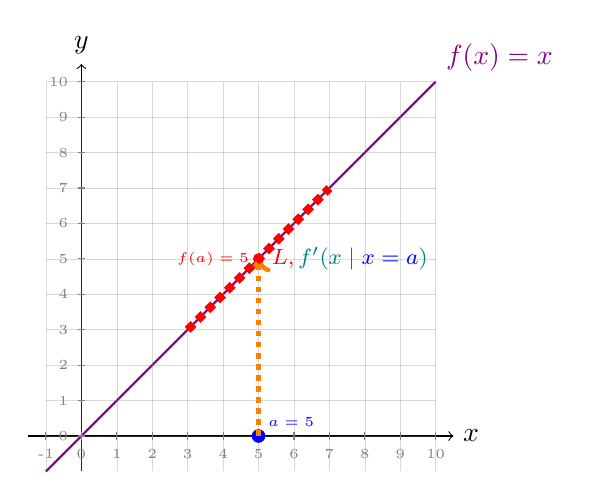
\begin{tikzpicture}[scale=0.45]
        % Draw axes
        \draw[->] (-1.5, 0) -- (10.5, 0) node[right] {\(x\)};
        \draw[->] (0, -1) -- (0, 10.5) node[above] {\(y\)};
  
        % Draw the line y = x in violet
        \draw[thick, violet, domain=-1:10] plot (\x, \x) node[above right] {\(f(x) = x\)};
  
        % Grid lines in gray
        \foreach \x in {-1,...,10}
          \draw[gray, very thin, opacity=0.3] (\x,-1) -- (\x,10);
        \foreach \y in {0,...,10}
          \draw[gray, very thin, opacity=0.3] (-1,\y) -- (10,\y);
  
        % Labels on axes in gray
        \foreach \x in {-1,0,...,10}
          \draw[gray] (\x,0.1) -- (\x,-0.1) node[below, gray] {\tiny \x};
        \foreach \y in {0,...,10}
          \draw[gray] (0.1,\y) -- (-0.1,\y) node[left, gray] {\tiny \y};
  
        % Blue dot at (5,0)
        \filldraw[blue] (5,0) circle (5pt) node[above right] {\tiny \(a = 5\)};
  
        % Red dot at (5, 5)
        \filldraw[red] (5,5) circle (4pt) node[left] {\tiny \(f(a) = 5\)};
  
        % Orange dotted arrow from (5,0) to (5,5)
        \draw[->, orange, line width=2pt, dotted] (5,0) -- (5,5);
  
        % Dotted red line from (3,3) to (7,7) with label
        \draw[red, dotted, line width=3pt] (3,3) -- (7,7) node[pos=0.5, right, red] {\footnotesize \(L, \textcolor{teal}{f'(x \mid \textcolor{blue}{x = a})} \)};
      \end{tikzpicture}
    \end{column}
    
  \end{columns}
\end{frame}


\begin{frame}{미분의 접근법: 기하학(Geometry) \( f(x) = x^2 \)}
  \begin{columns}
    \begin{column}{0.5\textwidth}
        \begin{itemize}
          \item 미분=함수의 기울기=접선의 기울기 \\
             미분은 접선의 기울기 $\Longleftrightarrow$ 접선의 기울기는 미분 \\
             미분계수는 함수의 순간 변화율=접선의 기울기
        \end{itemize}
    \end{column}
    \begin{column}{0.5\textwidth}
      % Add an image or diagram related to the geometric approach of differentiation
      % Example: A graph showing a function and its tangent line at a point
      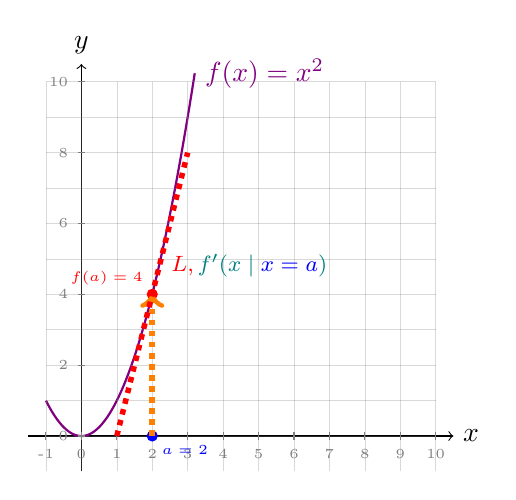
\begin{tikzpicture}[scale=0.45]
        % Draw axes
        \draw[->] (-1.5, 0) -- (10.5, 0) node[right] {\(x\)};
        \draw[->] (0, -1) -- (0, 10.5) node[above] {\(y\)};

        % Draw the function f(x) = x^2 in violet
        \draw[thick, violet, domain=-1:3.2, samples=100] plot (\x, {\x*\x}) node[right] {\(f(x) = x^2\)};

        % Grid lines in gray
        \foreach \x in {-1,...,10}
          \draw[gray, very thin, opacity=0.3] (\x,-1) -- (\x,10);
        \foreach \y in {0,...,10}
          \draw[gray, very thin, opacity=0.3] (-1,\y) -- (10,\y);

        % Labels on axes in gray
        \foreach \x in {-1,0,...,10}
          \draw[gray] (\x,0.1) -- (\x,-0.1) node[below, gray] {\tiny \x};
        \foreach \y in {0,2,...,10}
          \draw[gray] (0.1,\y) -- (-0.1,\y) node[left, gray] {\tiny \y};

        % Blue dot at (2, 0)
        \filldraw[blue] (2,0) circle (4pt) node[below right] {\tiny \(a = 2\)};

        % Red dot at (2, 4)
        \filldraw[red] (2,4) circle (4pt) node[above left] {\tiny \(f(a) = 4\)};

        % Orange dotted arrow from (2,0) to (2,4)
        \draw[->, orange, line width=2pt, dotted] (2,0) -- (2,4);

        % Tangent line: y = 4x - 4 (through (2,4), slope 4)
        \draw[red, dotted, thin, line width=2pt] (1, 0) -- (3, 8) 
          node[pos=0.6, right, red] {\footnotesize \(L, \textcolor{teal}{f'(x \mid \textcolor{blue}{x = a})} \)};
      \end{tikzpicture}
    \end{column}
    
  \end{columns}
\end{frame}


\begin{frame}{미분의 접근법: 기하학(Geometry) \( f(x) = x^2 \)}
  \begin{columns}
    \begin{column}{0.5\textwidth}
        \begin{itemize}
          \item 평균변화율: 구간 \( [a, b] \)에서 함수의 평균적 변화율 (delta y / delta x)
             \[ \frac{f(b)-f(a)}{b-a} \]
          \item 순간변화율: 특정 지점 \( x=a \)에서의 변화율 (미분계수) (dy / dx)
             \[ \lim_{h \to 0} \frac{f(a+h)-f(a)}{h} \]
        \end{itemize}
    \end{column}
    \begin{column}{0.5\textwidth}
      % Add an image or diagram related to the geometric approach of differentiation
      % Example: A graph showing a function and its tangent line at a point
      \begin{tikzpicture}[scale=0.45]
        % Draw axes
        \draw[->] (-1.5, 0) -- (10.5, 0) node[right] {\(x\)};
        \draw[->] (0, -1) -- (0, 10.5) node[above] {\(y\)};
      
        % Draw f(x) = 0.25 * x^2
        \draw[thick, violet, domain=0:6, samples=100] 
          plot (\x, {0.25*\x*\x}) 
          node[right] {\(f(x) = 0.25x^2\)};
      
        % Grid lines in gray
        \foreach \x in {-1,...,10}
          \draw[gray, very thin, opacity=0.3] (\x,-1) -- (\x,10);
        \foreach \y in {0,...,10}
          \draw[gray, very thin, opacity=0.3] (-1,\y) -- (10,\y);
      
        % Points a = 2 and b = 6
        \filldraw[blue] (2,1) circle (3pt) node[below left] {\tiny \(a=2\)};
        \filldraw[blue] (6,9) circle (3pt) node[above right] {\tiny \(b=6\)};
        \draw[thick, orange, dashed] (2,1) -- (6,9) 
          node[pos=0.5, above left, orange] {\small 평균 변화율: 2};
      
        % Point x = 2
        \filldraw[red] (4,4) circle (3pt) node[above left] {\tiny \(x = 2\)};
        \draw[->, orange, line width=1pt, dotted] (4,0) -- (4,4);
      
        % Tangent at x = 2: slope = 1, equation: y = x - 1
        \draw[red, dotted, very thick, domain=1:4] 
          plot (\x, {\x - 1}) 
          node[pos=0.9, above right, red] {\footnotesize \(L,\ f'(x) = 1\)};
      \end{tikzpicture}
      
    \end{column}
    
  \end{columns}
\end{frame}







% \section{미분의 풀이법}
% \begin{frame}{미분의 풀이법 : 기울기와 미분계수}
%   \begin{itemize}
%     \item askjdfkasdf
%   \end{itemize}
% \end{frame}



% \begin{frame}{다항함수의 미분법}
%   \begin{itemize}
%     \item 1차 함수 \( f(x)=ax+b \), 도함수는 \( f'(x)=a \)
%     \item 2차 함수 \( f(x)=ax^2+bx+c \), 도함수는 \( f'(x)=2ax+b \)
%     \item 3차 함수 \( f(x)=ax^3+bx^2+cx+d \), 도함수는 \( f'(x)=3ax^2+2bx+c \)
%   \end{itemize}
% \end{frame}




\section{함수에 따른 미분법}

\begin{frame}{함수에 따른 미분법: 공식}
  \begin{itemize}
    \item Constant (상수): \( \frac{\mathbf{d}}{\mathbf{d}x} c = 0 \)
    \item Polynomial: $ \frac{\mathbf{d}}{\mathbf{d}x} x^n = n \cdot x^{n-1}  $
    % \item Fraction: \( \left(\frac{f(x)}{g(x)}\right)'=\frac{f'(x)g(x)-f(x)g'(x)}{g(x)^2} \)
    % \item Exponential: \( (e^x)'=e^x \)
    % \item Logarithmic: \( (\ln x)'=\frac{1}{x} \)
  \end{itemize}
\end{frame}

% \begin{frame}{함수에 따른 미분법: Polynomial}
%   \begin{block}{$\frac{\mathbf{d}}{\mathbf{d}x} f(x) = \frac{\mathbf{d}}{\mathbf{d}x} (a\cdot x^n)$}
    
%   \end{block}
  
% \end{frame}


\begin{frame}{함수에 따른 미분법: Polynomial $f(x) = ax$}
  \begin{definition}[도함수]
    % 실수($\mathbb{R}$)의 어떤 함수 \textcolor{violet}{$f(x)$}가 정의되는 포인트 \textcolor{blue}{\emph{$x_0$}} 에서 \emph{미분가능(differentiable)} 하고, 정의역이 포인트 \textcolor{blue}{\emph{$x_0$}} 를 포함한다면, \textcolor{blue}{\emph{$x_0$}} 에서 \textcolor{red}{미분계수(순간변화율)} \textcolor{red}{\emph{$L$}} 은 \\
    \begin{equation*}
      \textcolor{red}{L} = \textcolor{teal}{\lim_{h \to 0} \frac{f(\textcolor{blue}{x_0}+h)-f(\textcolor{blue}{x_0})}{h}}
    \end{equation*}
  \end{definition}
  % 
  \begin{align*}
    & \textcolor{magenta}{f(x) = ax}, \quad \text{도함수: } f'(x) = \lim_{h \to 0} \frac{f(x+h)-f(x)}{h} \\
    & \text{도함수에 대입. 예를 들어, } \textcolor{magenta}{f(x+h) = a(x+h)} \\
    & \rightarrow f'(x) = \lim_{h \to 0} \frac{\textcolor{magenta}{a(x+h)}- \textcolor{magenta}{ax}}{h} \\
    \lim \text{계산} \rightarrow & = \lim_{h \to 0} \frac{ax + ah -ax}{h} = \lim_{h \to 0} \frac{ah}{h} = \lim_{h \to 0} a = a\\
  \end{align*}
  % 
\end{frame}


\begin{frame}{함수에 따른 미분법: Polynomial $f(x) = ax^2$}
  \begin{align*}
    & \textcolor{magenta}{f(x) = ax^2}, \quad \text{도함수: } f'(x) = \lim_{h \to 0} \frac{f(x+h)-f(x)}{h} \\
    & \text{도함수에 대입} \rightarrow f'(x) = \lim_{h \to 0} \frac{\textcolor{magenta}{a(x +h)^2} - \textcolor{magenta}{ax^2}}{h} \\
    & = \lim_{h \to 0} \frac{ax^2 + 2axh + ah^2 - ax^2}{h} \\
    & = \lim_{h \to 0} \frac{2axh + ah^2}{h} = \lim_{h \to 0} 2ax + \lim_{h \to 0} ah = 2ax + a \cdot 0 = 2ax \\
    & \therefore f'(x) = 2ax \\
    & f'(x \mid x=1) = 2a\cdot 1, \quad f'(x \mid x=2) = 4a
  \end{align*}
  % 
\end{frame}

\begin{frame}{함수에 따른 미분법: Polynomial $f(x) = \frac{1}{x}, f(x) = x^{-1}$}
  \begin{align*}
    & f(x) = \textcolor{magenta}{\frac{1}{x}} = x^{-1}, \quad \text{도함수:} f'(x) = \lim_{h \to 0} \frac{f(x+h)-f(x)}{h} \\
    & \text{도함수에 대입} \rightarrow f'(x) = \lim_{h \to 0} \frac{ \textcolor{magenta}{\frac{1}{x+h}} - \textcolor{magenta}{\frac{1}{x}}}{h} \\
    & = \lim_{h \to 0} \frac{\frac{x - (x + h)}{x(x+h)}}{h}  = \lim_{h \to 0} \frac{\frac{-h}{x(x+h)}}{h} = \lim_{h \to 0} \frac{-h}{hx(x+h)}   \\
    & = \lim_{h \to 0} \frac{-1}{x(x+h)} = \lim_{h \to 0} \frac{-1}{x^2+hx}   = \frac{-1}{x^2} \\
    & \therefore f'(x) = -\frac{1}{x^2} = {-1}x^{-2} \\
    & f'(x \mid x=1) = -1, \quad f'(x \mid x=2) = -\frac{1}{4}
  \end{align*}
\end{frame}



\begin{frame}{함수에 따른 미분법: Polynomial 예제}
  \begin{columns}
    \begin{column}{.5\textwidth}
      \begin{align*}
        & f(x) = a \cdot x^3 \\
        & f'(x)' = \\
      \end{align*}
      \begin{align*}
        & g(x) = \cdot x^{(-4)} \\
        & \frac{\mathbf{d}}{\mathbf{d}x}f(x) = \\
      \end{align*}    
    \end{column}
    % \begin{column}{.5\textwidth}
    %   \begin{align*}
    %     & f(x) = 2 \cdot x^2 + x  \\
    %     & f'(x) = \\
    %   \end{align*}
    %   \begin{align*}
    %     & f(x) = a \cdot x^{10} + b \cdot x^5 + c \cdot x^2 + d\\
    %     & f'(x) = \\
    %   \end{align*}    
    % \end{column}
  \end{columns}
\end{frame}

\begin{frame}{함수에 따른 미분법: Polynomial 예제}
  \begin{columns}
    % \begin{column}{.5\textwidth}
    %   \begin{align*}
    %     & f(x) = a \cdot x^3 \\
    %     & f'(x)' = \\
    %   \end{align*}
    %   \begin{align*}
    %     & g(x) = \cdot x^{(-4)} \\
    %     & \frac{\mathbf{d}}{\mathbf{d}x}f(x) = \\
    %   \end{align*}    
    % \end{column}
    \begin{column}{.5\textwidth}
      \begin{align*}
        & f(x) = 2 \cdot x^2 + x  \\
        & f'(x) = \\
      \end{align*}
      \begin{align*}
        & f(x) = a \cdot x^{10} + b \cdot x^5 + c \cdot x^2 + d\\
        & f'(x) = \\
      \end{align*}    
    \end{column}
  \end{columns}
\end{frame}






\section{곱의 미분}

\begin{frame}{곱의 미분}
  \begin{block}{곱의 미분법(= 나눗셈의 미분법)}
    \begin{align*}
      (f \cdot g)' = f' \cdot g + f \cdot g' \\
      \left(\frac{f}{g} \right)' = \frac{f' \cdot g - f \cdot g'}{g^2}
    \end{align*}
  \end{block}
\end{frame}


\begin{frame}{곱의 미분}
  \scalebox{0.85}{%
  \parbox{\linewidth}{%
  \begin{align*}
    & \text{함수 } \textcolor{blue}{f(x)}, \textcolor{red}{g(x)} \text{ 에 대해 } h(x) = \textcolor{blue}{f(x)}\textcolor{red}{g(x)} \text{ 라 하자} \\
    & h'(x) = \lim_{h \to 0} \frac{\textcolor{blue}{f(x+h)}\textcolor{red}{g(x+h)} - \textcolor{blue}{f(x)}\textcolor{red}{g(x)}}{h} \\
    \\
    & \textcolor{gray}{\text{두 항의 차를 직접 다루기 어렵기 때문에, 더하고 빼기}} \\
    & = \lim_{h \to 0} \frac{\textcolor{blue}{f(x+h)}\textcolor{red}{g(x+h)} - \textcolor{blue}{f(x)}\textcolor{red}{g(x+h)} + \textcolor{blue}{f(x)}\textcolor{red}{g(x+h)} - \textcolor{blue}{f(x)}\textcolor{red}{g(x)}}{h} \\
    & = \lim_{h \to 0} \left[ \frac{\textcolor{blue}{f(x+h)} - \textcolor{blue}{f(x)}}{h} \cdot \textcolor{red}{g(x+h)} + \textcolor{blue}{f(x)} \cdot \frac{\textcolor{red}{g(x+h)} - \textcolor{red}{g(x)}}{h} \right] \\
    \\
    & \text{극한은 각각 따로 가능하므로:} \\
    & = \left( \lim_{h \to 0} \frac{\textcolor{blue}{f(x+h)} - \textcolor{blue}{f(x)}}{h} \right) \cdot \left( \lim_{h \to 0} \textcolor{red}{g(x+h)} \right) + \textcolor{blue}{f(x)} \cdot \left( \lim_{h \to 0} \frac{\textcolor{red}{g(x+h)} - \textcolor{red}{g(x)}}{h} \right) \\
    & = \textcolor{blue}{f'(x)} \cdot \textcolor{red}{g(x)} + \textcolor{blue}{f(x)} \cdot \textcolor{red}{g'(x)} \\
    \\
    & \therefore \boxed{(\textcolor{blue}{f} \cdot \textcolor{red}{g})'(x) = \textcolor{blue}{f'(x)}\textcolor{red}{g(x)} + \textcolor{blue}{f(x)}\textcolor{red}{g'(x)}}
  \end{align*}
  }%
  }
\end{frame}

\begin{frame}{곱의 미분: 함수의 형태에 따라.}
  \begin{columns}
    \begin{column}{.5\textwidth}
      \begin{align*}
        & f(x) = a \cdot x , \quad g(x) = c \cdot x^3 \\
        & (f(x) \cdot g(x))' = \\
        % & \frac{\mathbf{d}}{\mathbf{d}x}(f(x) \cdot g(x)) = \\
      \end{align*}
      \begin{align*}
        & f(x) = x^2 , \quad g(x) = x^{-4} \\
        % & (f(x) \cdot g(x))' = \\
        & \frac{\mathbf{d}}{\mathbf{d}x}(f(x) \cdot g(x)) = \\
      \end{align*}
      % \begin{align*}
      %   & f(x) = a \cdot x^3 \\
      %   & f'(x)' = \\
      % \end{align*}
      % \begin{align*}
      %   & g(x) = \cdot x^{(-4)} \\
      %   & \frac{\mathbf{d}}{\mathbf{d}x}f(x) = \\
      % \end{align*}    
    \end{column}
    % \begin{column}{.5\textwidth}
    %   \begin{align*}
    %     & f(x) = x^2 , \quad g(x) = 2 \cdot x^2 + x \\
    %     & (f(x) \cdot g(x))' = \\
    %     % & \frac{\mathbf{d}}{\mathbf{d}x}(f(x) \cdot g(x)) = \\
    %   \end{align*}
    %   \begin{align*}
    %     & f(x) = x^2 + x \\
    %     & g(x) = a \cdot x^{10} + b \cdot x^5 + c \cdot x^2 + d \\
    %     & (f(x) \cdot g(x))' = \\
    %     % & \frac{\mathbf{d}}{\mathbf{d}x}(f(x) \cdot g(x)) = \\
    %   \end{align*}  
    % \end{column}
  \end{columns}
\end{frame}


\begin{frame}{곱의 미분: 함수의 형태에 따라.}
  \begin{columns}
    % \begin{column}{.5\textwidth}
    %   \begin{align*}
    %     & f(x) = a \cdot x , \quad g(x) = c \cdot x^3 \\
    %     & (f(x) \cdot g(x))' = \\
    %     % & \frac{\mathbf{d}}{\mathbf{d}x}(f(x) \cdot g(x)) = \\
    %   \end{align*}
    %   \begin{align*}
    %     & f(x) = x^2 , \quad g(x) = x^{-4} \\
    %     % & (f(x) \cdot g(x))' = \\
    %     & \frac{\mathbf{d}}{\mathbf{d}x}(f(x) \cdot g(x)) = \\
    %   \end{align*}
    %   % \begin{align*}
    %   %   & f(x) = a \cdot x^3 \\
    %   %   & f'(x)' = \\
    %   % \end{align*}
    %   % \begin{align*}
    %   %   & g(x) = \cdot x^{(-4)} \\
    %   %   & \frac{\mathbf{d}}{\mathbf{d}x}f(x) = \\
    %   % \end{align*}    
    % \end{column}
    \begin{column}{.5\textwidth}
      \begin{align*}
        & f(x) = x^2 , \quad g(x) = 2 \cdot x^2 + x \\
        & (f(x) \cdot g(x))' = \\
        % & \frac{\mathbf{d}}{\mathbf{d}x}(f(x) \cdot g(x)) = \\
      \end{align*}
      \begin{align*}
        & f(x) = x^2 + x \\
        & g(x) = a \cdot x^{10} + b \cdot x^5 + c \cdot x^2 + d \\
        & (f(x) \cdot g(x))' = \\
        % & \frac{\mathbf{d}}{\mathbf{d}x}(f(x) \cdot g(x)) = \\
      \end{align*}  
    \end{column}
  \end{columns}
\end{frame}



\section{합성함수의 미분: Chain Rule}


\begin{frame}{합성함수의 미분: Chain Rule}
  \begin{block}{Chain Rule}
    \begin{align*}
      & h = {f} \circ {g} \text{ 인 합성함수 } h \text{ 라면} \\
      & h' \text{ 혹은 } \mathbf{d} h  = ( {f} \circ {g} )' = {f'}({g}) \cdot {g'} \\[1em]
      & \text{e.g. } h = {f} \circ {g} = f(g(x)) \\
      & \frac{\mathbf{d}}{\mathbf{d}x} h = \frac{\mathbf{d}}{\mathbf{d}x} f(g(x)) = \frac{\mathbf{d}}{\mathbf{d}g(x)} f(g(x)) \cdot \frac{\mathbf{d}}{\mathbf{d}x} g(x) \\
      & \text{이때, } u = g(x) \text{ 로 치환하면, 편리해 짐. 'u-substitution'이라는 미분 테크닉.} \\
      & \text{e.g. } u = g(x) \rightarrow h = {f} \circ {g} = f(u), \quad  \\
      & \frac{\mathbf{d}}{\mathbf{d}x} h = \frac{\mathbf{d}}{\mathbf{d}x} f(u) = \frac{\mathbf{d}}{\mathbf{d}u} f(u) \cdot \frac{\mathbf{d}u}{\mathbf{d}x}  \\
    \end{align*}
  \end{block}
\end{frame}

\begin{frame}{합성함수의 미분: Chain Rule}
  \scalebox{0.85}{%
  \parbox{\linewidth}{%
  \begin{align*}
    % & \text{합성함수 } h(x) = \textcolor{blue}{f(}\textcolor{red}{g(x)}\textcolor{blue}{)} \text{ 에 대해 도함수를 정의로 구함} \\
    & h'(x) = \lim_{h \to 0} \frac{\textcolor{blue}{f(}\textcolor{red}{g(x+h)}\textcolor{blue}{)} - \textcolor{blue}{f(}\textcolor{red}{g(x)}\textcolor{blue}{)}}{h} \\
    % \\
    % & \textcolor{gray}{\text{(중간 단계: 분모에 } \textcolor{red}{g(x+h) - g(x)} \textcolor{gray}{ 를 곱하고 나누기)}} \\
    & = \lim_{h \to 0} \left[ \frac{\textcolor{blue}{f(}\textcolor{red}{g(x+h)}\textcolor{blue}{)} - \textcolor{blue}{f(}\textcolor{red}{g(x)}\textcolor{blue}{)}}{\textcolor{red}{g(x+h) - g(x)}} \cdot \frac{\textcolor{red}{g(x+h) - g(x)}}{h} \right] \\
    & \text{앞부분은 마치 } \frac{\Delta f(g(x))}{\Delta g(x)} \text{ 인데 $\Delta \to 0 $ 이면 미분의 정의} \\
    & \text{극한을 각각 분리하고, u를 치환하면:} \\
    % & \textcolor{gray}{\text{복잡한 함수의 극한을 다루기 위해 다음과 같이 치환한다:}} \\
    & \textcolor{black}{u = g(x+h)} \quad \Rightarrow \quad \textcolor{black}{u \to g(x)} \text{ as } h \to 0 \text{ (왜냐하면 } \textcolor{black}{g} \text{ 가 연속이므로)} \\
    & = \left( \lim_{\textcolor{red}{u} \to \textcolor{red}{g(x)}} \frac{\textcolor{blue}{f(}\textcolor{red}{u}\textcolor{blue}{)} - \textcolor{blue}{f(}\textcolor{red}{g(x)}\textcolor{blue}{)}}{\textcolor{red}{u - g(x)}} \right) \cdot \left( \lim_{h \to 0} \frac{\textcolor{red}{g(x+h)} - \textcolor{red}{g(x)}}{h} \right) \\
    & = \textcolor{blue}{f'}(\textcolor{red}{g(x)}) \cdot \textcolor{red}{g'(x)} \\
    % \\
    % & \therefore \boxed{( \textcolor{blue}{f} \circ \textcolor{red}{g} )'(x) = \textcolor{blue}{f'}(\textcolor{red}{g(x)}) \cdot \textcolor{red}{g'(x)}}
  \end{align*}
  }%
  }
\end{frame}





\begin{frame}{합성함수의 미분: 함수의 형태에 따라.}
  \begin{columns}
    \begin{column}{.5\textwidth}
      \begin{align*}
        & f(x) = a \cdot x , \quad g(x) = c \cdot x^3 \\
        & h = {f} \circ {g} = \\ 
        & h' =  ( {f} \circ {g} )' = \\
        % & \frac{\mathbf{d}}{\mathbf{d}x}(f(x) \cdot g(x)) = \\
      \end{align*}
      \begin{align*}
        & f(x) = x^2 , \quad g(x) = x^{-4} \\
        % & (f(x) \cdot g(x))' = \\
        & h = {f} \circ {g} = \\ 
        & \frac{\mathbf{d}}{\mathbf{d}x} h = \frac{\mathbf{d}}{\mathbf{d}x}( {f} \circ {g} ) = \\
      \end{align*} 
    \end{column}
    % \begin{column}{.5\textwidth}
    %   \textcolor{gray}{      
    %   \begin{align*}
    %     & f(x) = x^2 , \quad g(x) = 2 \cdot x^2 + x \\
    %     & ( {f} \circ {g} )' = \\
    %     % & \frac{\mathbf{d}}{\mathbf{d}x}(f(x) \cdot g(x)) = \\
    %   \end{align*}
    %   \begin{align*}
    %     & f(x) = x^2 + x \\
    %     & g(x) = a \cdot x^{10} + b \cdot x^5 + c \cdot x^2 + d \\
    %     & ( {f} \circ {g} )' = \\
    %     % & \frac{\mathbf{d}}{\mathbf{d}x}(f(x) \cdot g(x)) = \\
    %   \end{align*}
    %   } 
    % \end{column}
  \end{columns}  
\end{frame}


\begin{frame}{합성함수의 미분: 함수의 형태에 따라.}
      \begin{align*}
        & f(x) = x^2 , \quad g(x) = 2 \cdot x^2 + x \\
        & h = {f} \circ {g} = \\ 
        & h' = ( {f} \circ {g} )' = \\
        % & \frac{\mathbf{d}}{\mathbf{d}x}(f(x) \cdot g(x)) = \\
      \end{align*}
\end{frame}

\begin{frame}{합성함수의 미분: 함수의 형태에 따라.}
      \begin{align*}
        & f(x) = x^{20} \\
        & g(x) = x^{a} + x^{b} + c \\
        & h = {f} \circ {g} = \\ 
        & h' =  ( {f} \circ {g} )' = \\
        % & \frac{\mathbf{d}}{\mathbf{d}x}(f(x) \cdot g(x)) = \\
      \end{align*}
\end{frame}




% \begin{frame}{Chain Rule의 핵심 치환: \( u = g(x+h) \)}
%   \scalebox{0.85}{%
%   \parbox{\linewidth}{%
%   \begin{align*}
%     & h'(x) = \lim_{h \to 0} \frac{\textcolor{blue}{f(}\textcolor{red}{g(x+h)}\textcolor{blue}{)} - \textcolor{blue}{f(}\textcolor{red}{g(x)}\textcolor{blue}{)}}{h} \\
%     \\
%     & \textcolor{gray}{\text{복잡한 함수의 극한을 다루기 위해 다음과 같이 치환한다:}} \\
%     & \textcolor{red}{u = g(x+h)} \quad \Rightarrow \quad \textcolor{red}{u \to g(x)} \text{ as } h \to 0 \text{ (왜냐하면 } \textcolor{red}{g} \text{ 가 연속이므로)} \\
%     \\
%     & \text{그러면 위의 극한은 다음과 같이 바뀐다:} \\
%     & \lim_{h \to 0} \left( \frac{\textcolor{blue}{f(}\textcolor{red}{g(x+h)}\textcolor{blue}{)} - \textcolor{blue}{f(}\textcolor{red}{g(x)}\textcolor{blue}{)}}{\textcolor{red}{g(x+h)} - \textcolor{red}{g(x)}} \cdot \frac{\textcolor{red}{g(x+h)} - \textcolor{red}{g(x)}}{h} \right) \\
%     & \quad = \left( \lim_{\textcolor{red}{u} \to \textcolor{red}{g(x)}} \frac{\textcolor{blue}{f(u)} - \textcolor{blue}{f(g(x))}}{\textcolor{red}{u - g(x)}} \right) \cdot \left( \lim_{h \to 0} \frac{\textcolor{red}{g(x+h)} - \textcolor{red}{g(x)}}{h} \right) \\
%     \\
%     & \quad = \textcolor{blue}{f'(g(x))} \cdot \textcolor{red}{g'(x)}
%   \end{align*}
%   }%
%   }
% \end{frame}




% \begin{frame}%{합성함수의 미분: 함수의 형태에 따라.}
  
% \end{frame}






\end{document}
